% Beamer theme tmeplate - Quito light
% Author: Sofia Jijon (https://sjijon.github.io)
% Last Update: Sept 10, 2021
% Latest Version: https://github.com/sjijon/TeX-templates/tree/main/Beamer%20presentations/beamerthemequito-light


\documentclass[serif,10pt, aspectratio=169]{beamer}
\title[Causal Inference]{Smart City Construction: \\Analysis based on \\PSM-DiD and Machine Learning}
\date[\today]{\today}
\author[CK.Tian \& ZY.Li]{Presenter:\\Chenkai Tian 2211333\\Zeyu Li 2212026}
\institute{School of Finance, Nankai University}

\usepackage{pgfpages}
\usepackage{booktabs}
\usepackage{float}
\usepackage{graphicx}
\usepackage{subcaption}
\usepackage{xcolor}
\usepackage{array}
\usepackage{dcolumn}
\usepackage{caption}
\usepackage{tcolorbox}

\setbeameroption{hide notes}
%\setbeameroption{show notes on second screen=right}

\usetheme{quito-light}

\begin{document}
%_____________________________________________________
% Title page
\frame[plain]{
\titlepage
}
%_____________________________________________________
% ToC
\frame{{Table of contents}
\tableofcontents
}
%_____________________________________________________
% 
\section{Section 1}
\subsection{Subsection 1.1 Settings}

\frame{{Section 1}
{Framework}

\begin{figure}[H]
    \centering
    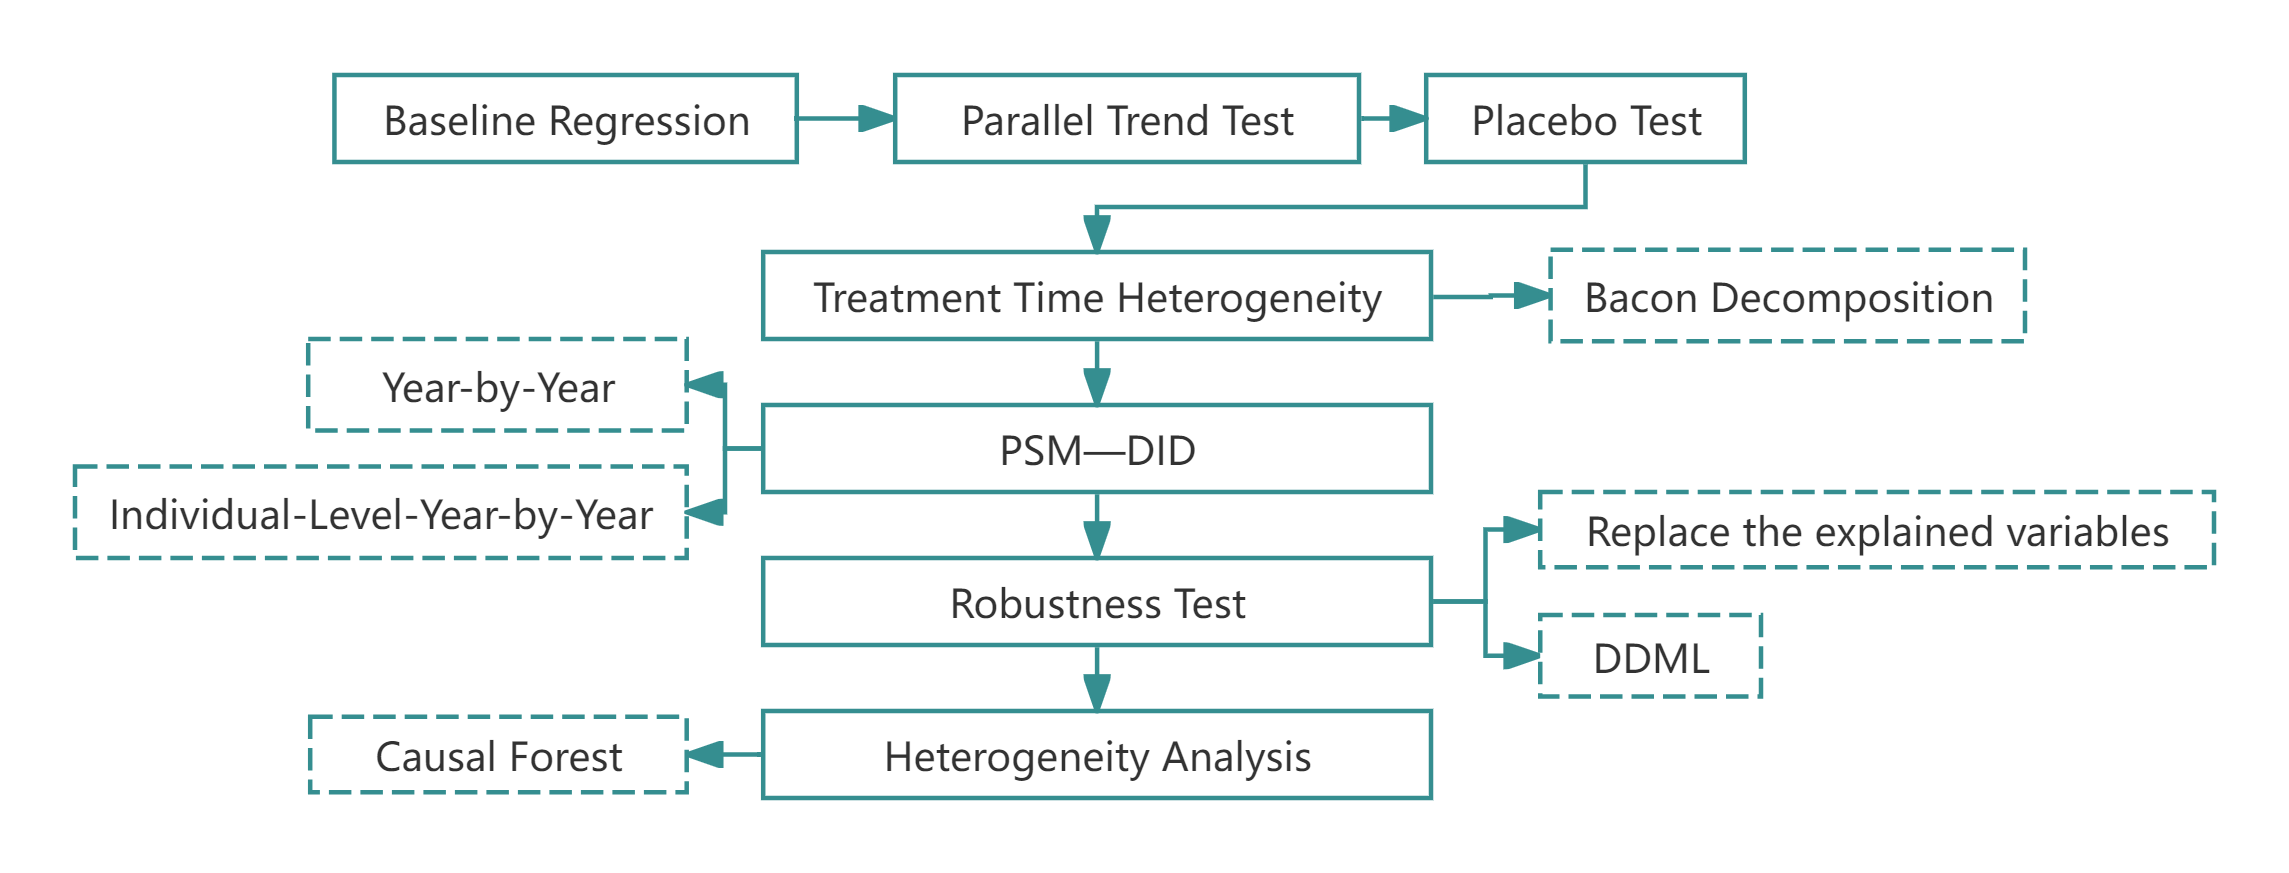
\includegraphics[width=\textwidth]{beamerthemequito-light/framework.jpg}
    \caption{General Framework}
    \label{fig:frame}  
\end{figure}
}

\frame{{Section 1} 
{Background \& Motivation}

\begin{itemize}
    \item We are faced with environmental pollution challenges brought by urbanization.
    \item The Chinese government has made significant efforts, among which Smart City Construction stands out as a policy tool.
\begin{itemize}
     \item[$\ast$] The first and second batch of pilot cities were announced in 2013.
     \item[$\ast$] The third batch of pilot cities was announced in 2015.
\end{itemize}
    \item We consider Smart City Construction policy in China as a quasi-natural experiment.
    \item The initiation of SCC since 2013 represents an exogenous policy shock to urban pollution emissions $\rightarrow$ Causal Inference!
\end{itemize}
}


\frame{{Section 1} 
{Dataset} 

\begin{itemize} 
\item Data is selected from "China Urban Statistical Yearbook".
\item We utilize a balanced panel dataset of 298 cities, with 119 smart city pilots.
\item A total of 5066 observations spanning from 2003 to 2019
\end{itemize}
}

\frame{{Section 1} 
{Dataset} 

\begin{figure}[H]
    \centering
    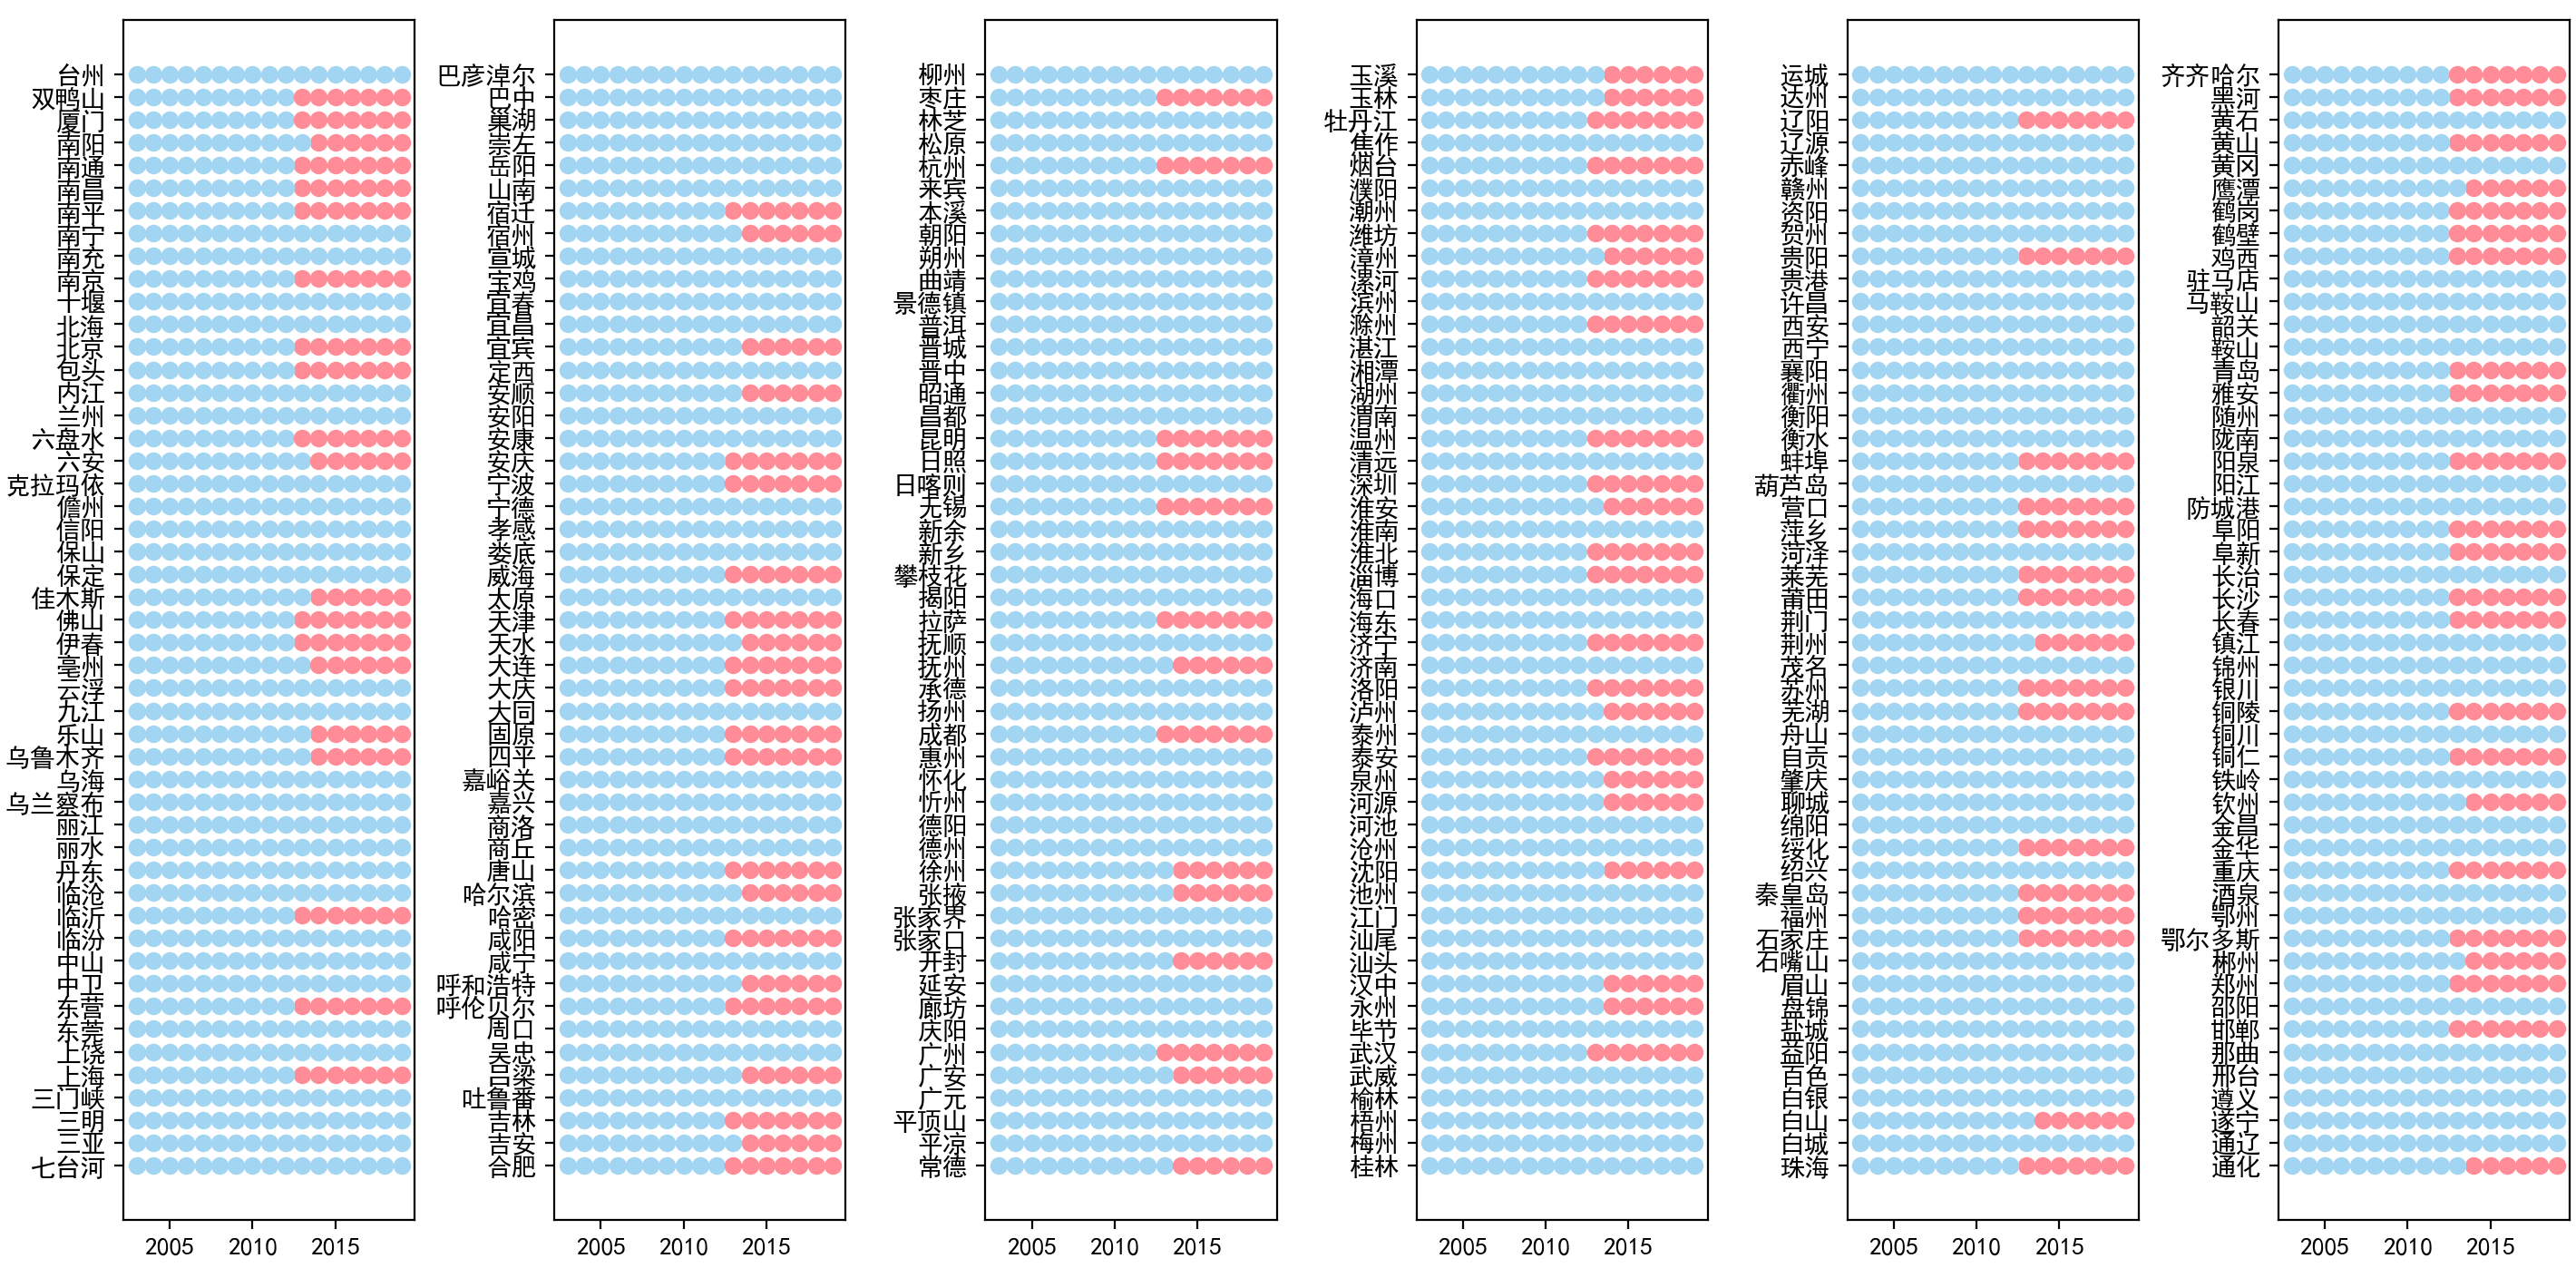
\includegraphics[width=0.9\textwidth]{beamerthemequito-light/pilot.jpg}  
    \caption{Time chart for SCC}
    \label{fig:pilot}  
\end{figure}
}

\frame{{Section 1} 
{Variables} 

\begin{table}[htbp]
\centering
\scalebox{0.85}{
\begin{tabular}{ccp{6cm}}
\toprule
 & Variable & Measurement \\
\midrule
Dependent Variable & pollution & Industrial wastewater, sulfur dioxide, and industrial smoke assessed using the entropy weight method. \\
Independent Variable & SCC & Whether it is a pilot city
for SCC \\
Control Variable & ln\_GDP & Natural logarithm of GDP \\
 & government\_intervention & Ratio of government fiscal
expenditure to GDP \\
 & urbanization\_level & Ratio of population to
registered population \\
 & financial\_development & Ratio of outstanding loans
of financial institutions to
GDP \\
 & population\_density & Ratio of registered urban
population to administrative area \\
 & education\_level & Natural logarithm of the
number of college students \\
\bottomrule
\end{tabular}
}
\end{table}
}

\frame{{Section 1} 
{Entropy Weight Method}


1.Standardize each emission indicator:


$$
    X_{i j t}^{\prime}=\frac{x_{i j t}-\min \left(x_{m j t}\right)}{\max \left(x_{m j t}\right)-\min \left(x_{m j t}\right)}
$$


2.Calculate the proportion $P_{i j t}$ of the $i$-th entity's value for the $j$-th indicator in the $t$-th year:

$$
P_{i j t}=\frac{X_{i j t}^{\prime}}{\sum_{i=1}^m X_{i j t}^{\prime}}\left(0 \leq P_{i j t} \leq 1\right)
$$
}

\frame{{Section 1} 
{Entropy Weight Method}

3.Compute the entropy value $e_{jt}$ for the $j$-th indicator:

$$
e_{j t}=-\frac{1}{\ln m} \sum_{i=1}^m P_{i j t} \ln P_{i j t}\left(0 \leq e_{j t} \leq 1\right)
$$

4.Assign the weight value $W_{jt}$ for the $j$-th indicator:

$$
W_{j t}=\frac{g_{j t}}{\sum_{j=1}^n g_{j t}}, g_{j t}=1-e_{j t}\left(0 \leq g_{j t} \leq 1, W_1+W_2+\bullet \bullet \bullet +W_j=1\right)
$$
}

\frame{{Section 1} 
{Entropy Weight Method}
5.Obtain the urban pollution emission for each city $i$:

$$
Poll_{i t}=\sum_{j=1}^n W_{j t} \times P_{i j t}
$$

}

\frame{{Section 1} 
{Smart City Construction}

\begin{itemize}
    \item $SCC$ is defined as the product of two dummy variables:
\end{itemize}

$$
SCC = smart \times post
$$

\begin{itemize}
    \item If a city is set as smart construction city, $smart$ takes the value of 1 as the treatment group, otherwise takes 0 as the control group.
    \item The time dummy variables $post$ before and after SCC are
assigned values of 0 and 1

\end{itemize}
}

\frame{{Section 1} 
{Correlation Matrix}

\begin{figure}[H]
    \centering
    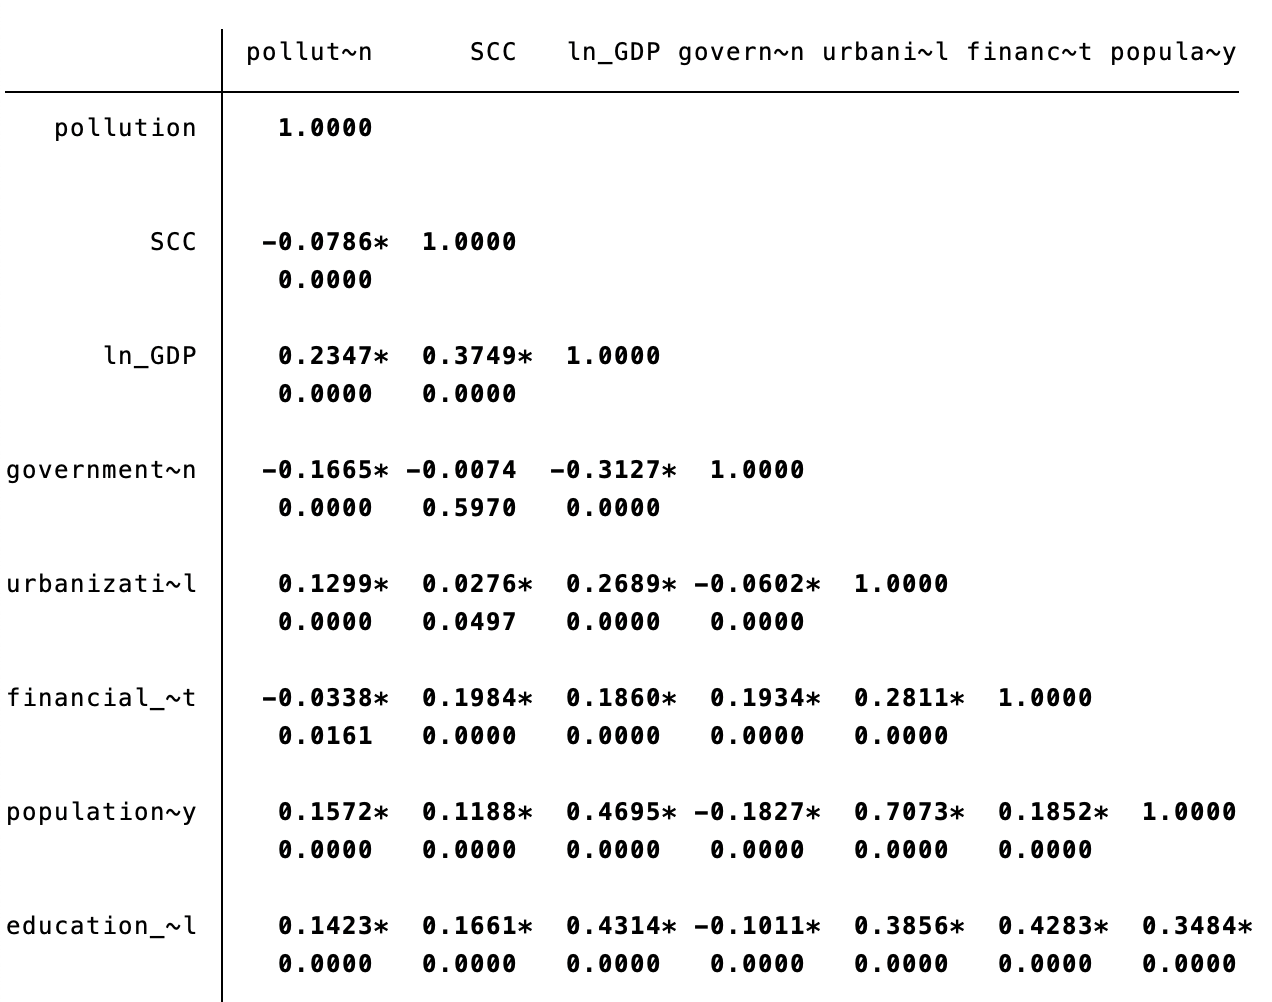
\includegraphics[width=0.5\textwidth]{beamerthemequito-light/Correlation.png}  
    \label{fig:Correlation}  
\end{figure}


Remark:The above table shows the correlation coefficients among variables,
showcasing small yet significant values, indicating the absence of multicollinearity.

}

\frame{{Section 1} 
{Jarque-Bera Test}

\begin{figure}[H]
    \centering
    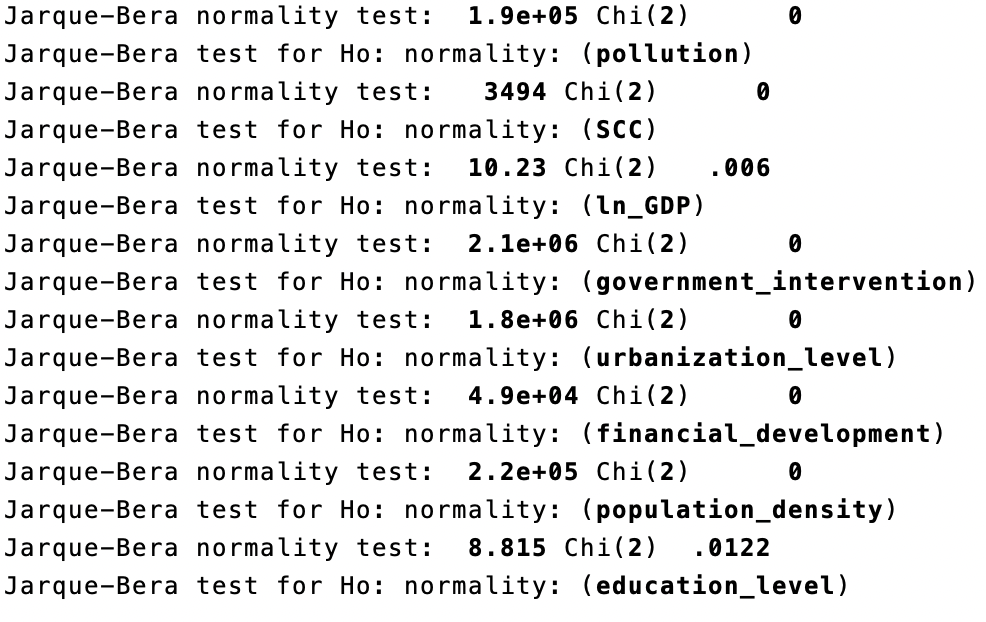
\includegraphics[width=0.5\textwidth]{beamerthemequito-light/JB.png}  
    \label{fig:JB}  
\end{figure}

Remark:The Jarque-Bera test yields p-values of 0,
rejecting normal distribution of the data. Given that the observations constitute large-sample data, deviations from normality are unlikely to significantly impact the regression outcomes.

}

\subsection{Subsection 1.2 Baseline Regression}
\frame{{Section 1} 
{Baseline Regression: Multi-period DiD}

We adopt the following regression model:

$$
Poll_{i t}=\beta_0+\beta_1 SSC_{i t}+\beta_2 Control_{i t}+ u_i+ \eta_t+\epsilon_{i t}
$$
where $i$ and $t$ represent the city and year, respectively. $\beta_1$ captures the effect of SCC on urban pollution levels. $u_i$ and $\eta_t$ represent the fixed effects for controlling cities and years respectively. $\epsilon_{it}$ is the error term.
}

\frame{{Section 1} 
{Baseline Regression: Results}

\begin{table}[htbp]
\centering
\resizebox{0.55\textwidth}{!}{
\begin{tabular}{lcccccc}
& \textbf{Without controls} & \textbf{With controls} \\

\hline
\textbf{SCC}                &      -0.200***&      -0.198***\\
                    &    (0.0725)   &    (0.0758)   \\
government\_intervention&               &     -0.0333   \\
                    &               &    (0.0954)   \\
urbanization\_level  &               &       0.144   \\
                    &               &     (0.152)   \\

financial\_development&               &      0.0123   \\
                    &               &    (0.0475)   \\

population\_density  &               &       0.861   \\
                    &               &     (7.212)   \\

education\_level     &               &     -0.0329   \\
                    &               &    (0.0203)   \\

Constant            &      0.0911***&      -3.141*  \\
                    &    (0.0342)   &     (1.718)   \\
\hline
Observations        &        5066   &        5066   \\
$R^2$                 &       0.322   &       0.328   \\
Year FE & Y & Y\\
City FE & Y & Y\\
\hline
\end{tabular}
}
\label{tab:BR}
\end{table}
}


\subsection{Subsection 1.3 Parallel Trend Test}
\frame{{Section 1} 
{Parallel Trend Test}

\begin{itemize}
    \item Meeting the parallel trend assumption $\rightarrow$ The Validity of DiD model
    \item We employ the following dynamic regression model:
\end{itemize}

$$
Poll_{i t}=\beta_0+\sum_{t=2}^{t=5}\alpha_{t} Pre_{i t}+ \sum_{t=0}^{t=5} \beta_{t}Post_{it} + \gamma Control_{i t}+ u_i+ \eta_t+\epsilon_{i t}
$$

\begin{itemize}
    \item $Pre_1$ is dropped to avoid perfect collinearity.
\end{itemize}

}
\frame{{Section 1} 
{Parallel Trend Test: Results}

\begin{figure}[H]
    \centering
    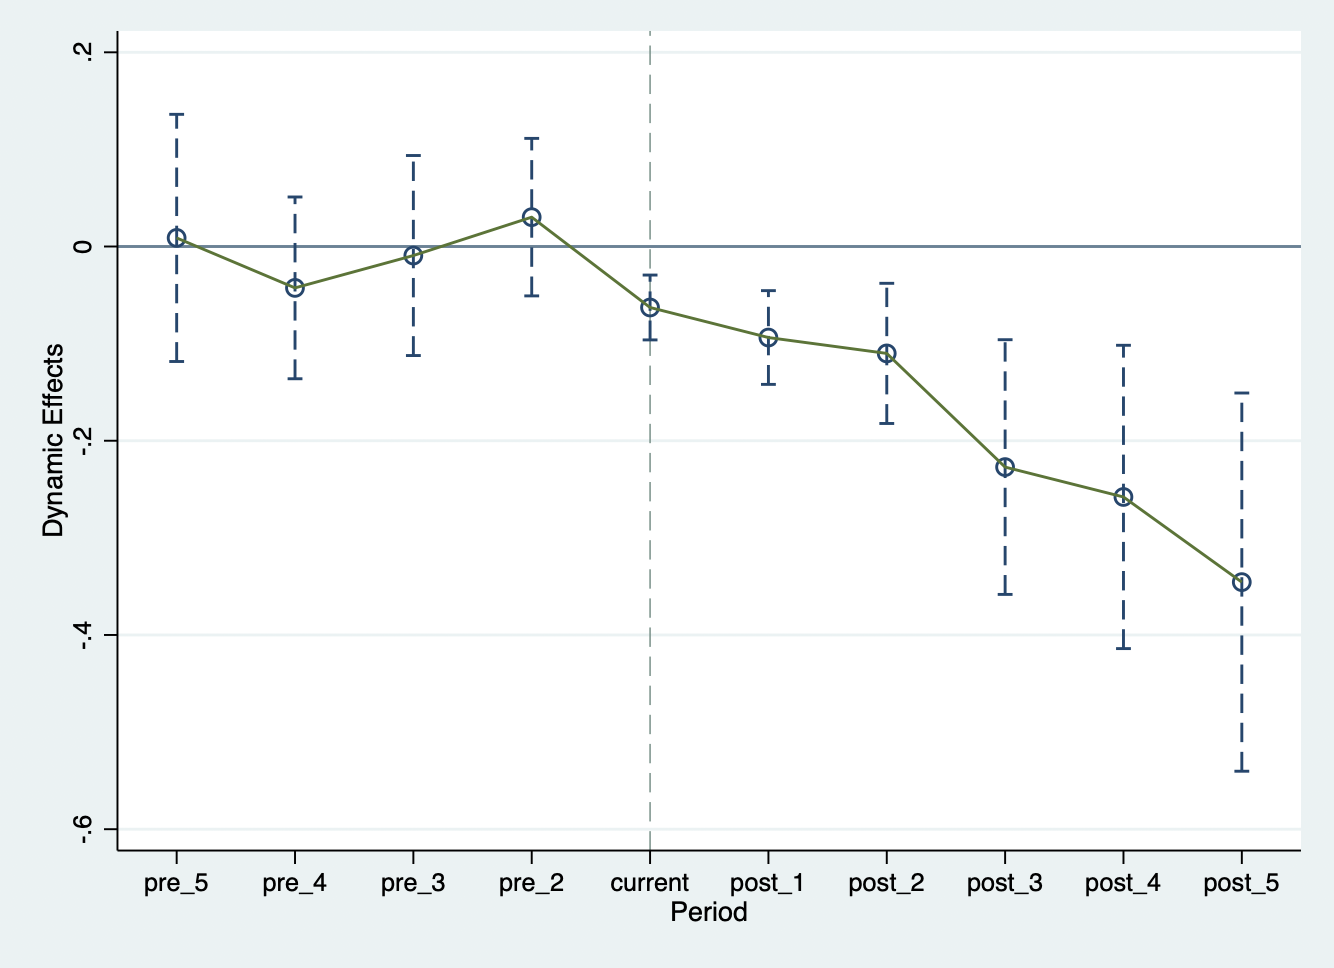
\includegraphics[width=0.6\textwidth]{beamerthemequito-light/Parallel Trend.png}  
    \label{fig:Parallel Trend}  
\end{figure}

}

\subsection{Subsection 1.4 Placebo Test}
\frame{{Section 1} 
{Placebo Test}

\begin{itemize}
    \item The estimation results may be
susceptible to interference from other random factors.
    \item It is imperative to conduct a placebo test by randomly generating pseudo-treatment group cities and virtual time variables!
\end{itemize}

}

\frame{{Section 1} 
{Placebo Test: Results}

\begin{figure}[H]
    \centering
    \caption{Placebo Tests with different repititions}
    \begin{subfigure}[b]{0.45\textwidth}
        \centering
        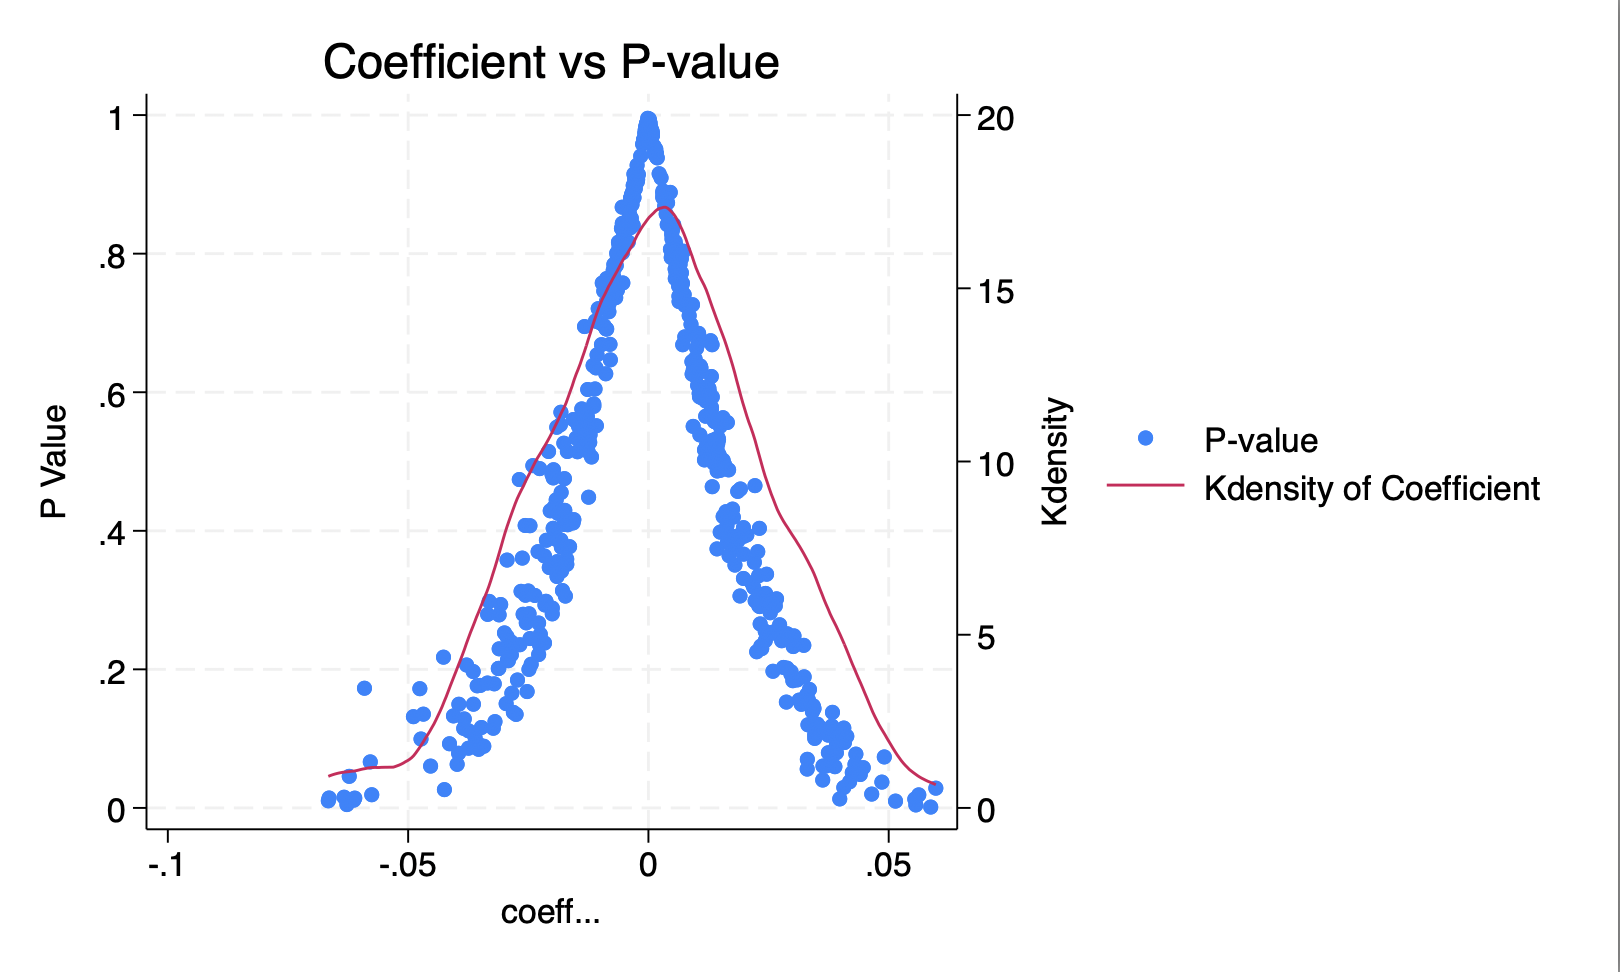
\includegraphics[width=\textwidth]{beamerthemequito-light/500.png}
        \caption{500 repititions}
        \label{fig:Placebo1}
    \end{subfigure}
    \hfill
    \begin{subfigure}[b]{0.45\textwidth}
        \centering
        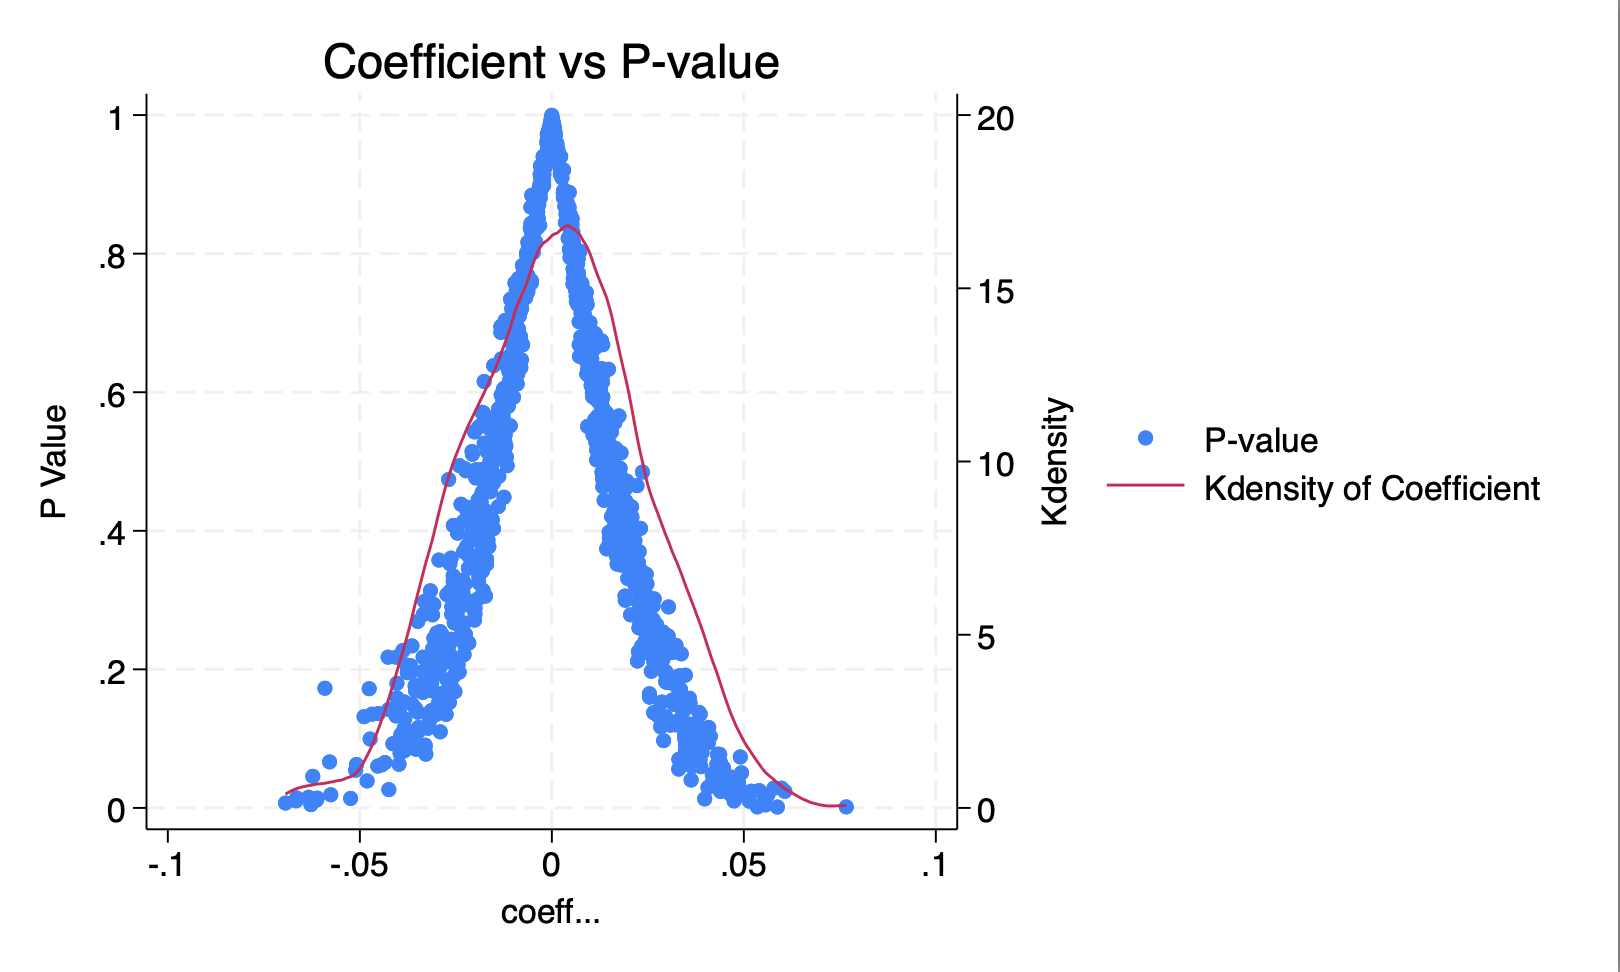
\includegraphics[width=\textwidth]{beamerthemequito-light/1000.png}
        \caption{1000 repititions}
        \label{fig:Placebo2}
    \end{subfigure}
    \label{fig:Placebo}
\end{figure}

The figures illustrate that the estimated coefficients predominantly
cluster around zero, with the majority of regression p-values exceeding
0.1, indicating non-significant results.
}

\subsection{Subsection 1.5 Bacon Decomposition}
\frame{{Section 1} 
{Bacon Decomposition}

We also conduct the following Bacon Decomposition:
$$
\begin{gathered}
\sum_t s_t+\sum_{e t \neq u t} \sum_{l t>e t}\left(s_{e t}+s_{l t}\right)=1 \\
\hat{\beta}^{D I D}=\sum_t s_t \hat{\beta}_{t, u t}^{D I D}+\sum_{e t \neq u t} \sum_{l t>e t}\left(s_{e t} \hat{\beta}_{e t, y u t}^{D I D}+s_{l t} \hat{\beta}_{l t, e t}^{D I D}\right)
\end{gathered}
$$
}

\frame{{Section 1} 
{Bacon Decomposition}
\begin{figure}[H]
    \centering
    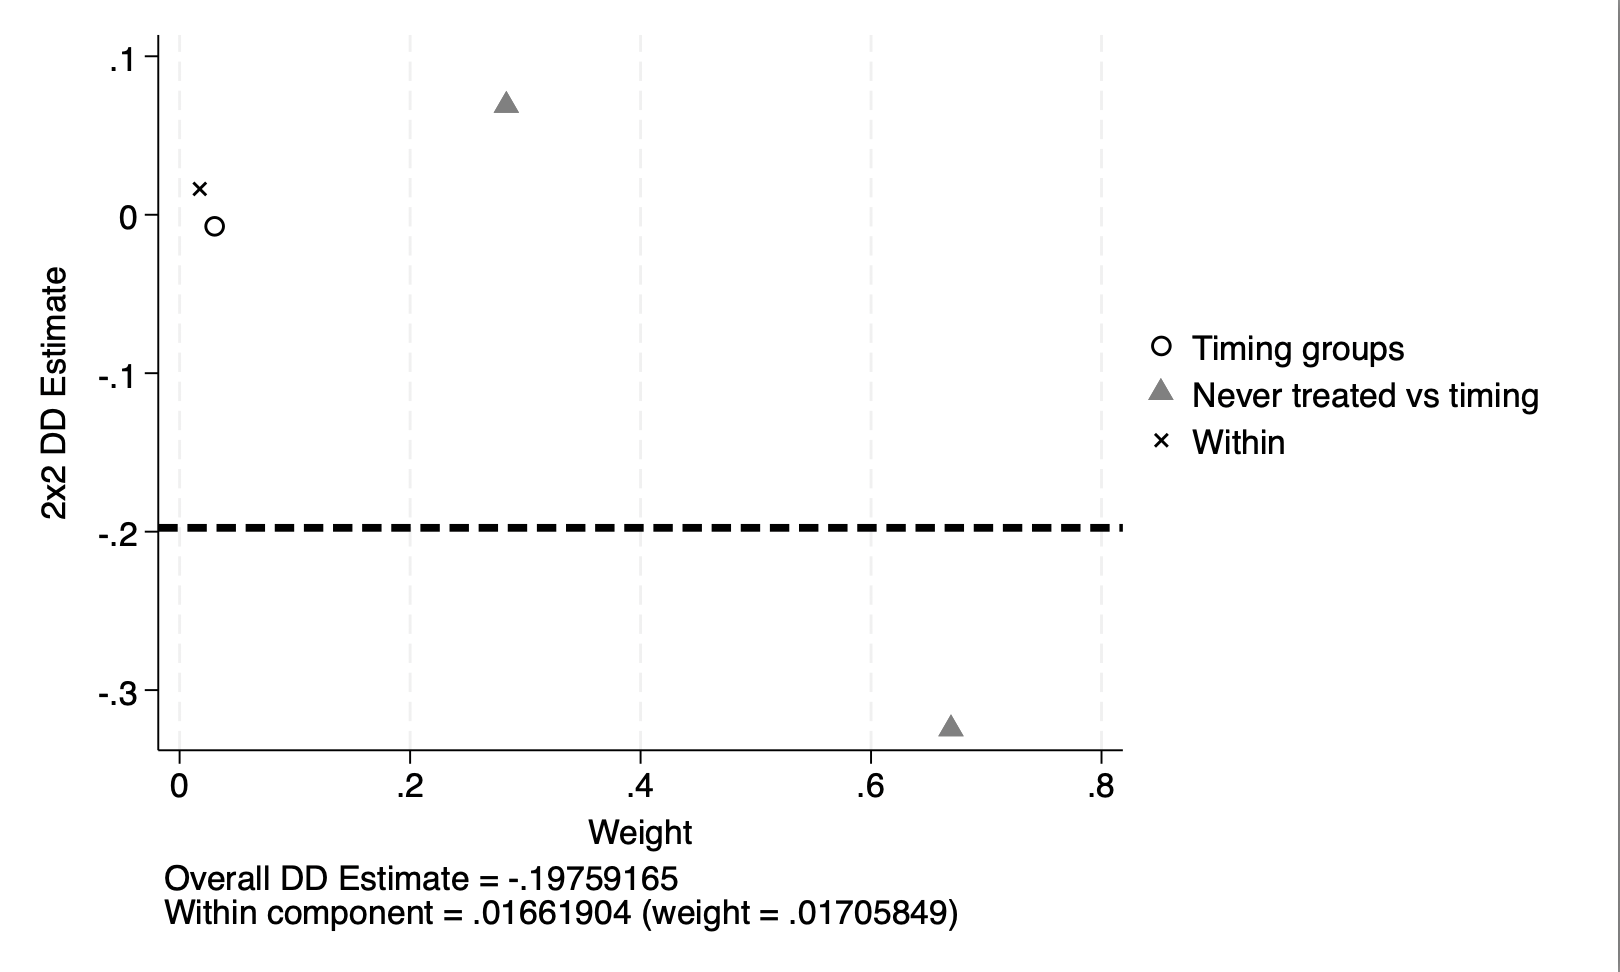
\includegraphics[width=0.8\textwidth]{beamerthemequito-light/Bacon1.png}  
    \label{fig:Bacon Decomposition}  
\end{figure}
}

\frame{{Section 1} 
{Bacon Decomposition}
\begin{figure}[H]
    \centering
    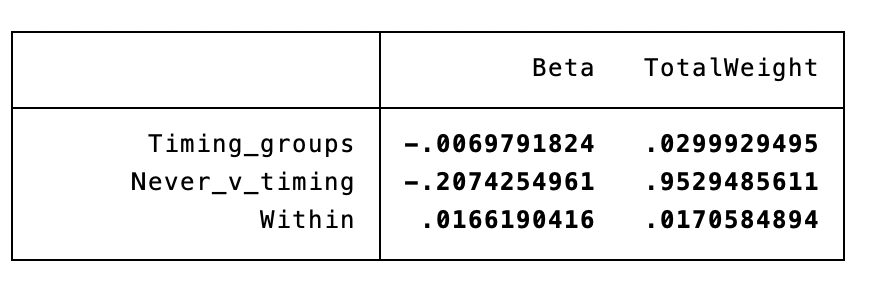
\includegraphics[width=0.7\textwidth]{beamerthemequito-light/Bacon2.png}  
    \label{fig:Bacon Decomposition}  
    \caption{Bacon Decomposition}
\end{figure}

}
\subsection{Subsection 1.6 PSM-DiD}
\frame{{Section 1} 
{PSM-DiD}

\begin{itemize}
    \item Governments may choose cities with relatively high pollution emissions for pilot projects, sample selection bias may arise.
    \item To mitigate estimation biases resulting from selection bias, the PSM-DiD model is used to test the estimated results
    \item However a number of problems can arise if we simply apply the same matching methods to our balanced panel dataset!(e.g.Self-selection)
    \item We therefore employ the following two matching methods that are more appropriate for \textcolor{red}{panel data}.
\end{itemize}
}

\frame{{Section 1} 
{Year-by-Year Matching}

\begin{itemize}
    \item Year-by-Year Matching is a propensity score matching (PSM) method used for panel data, where matching is done for treatment and control groups based on their treatment status in each year.
    \item Year-by-Year Matching is conducted through the following steps:
\end{itemize}

\begin{enumerate}
    \item Compute the propensity scores for all units in each year.
    \item Match the treatment group to the most similar control group based on the propensity scores.
    \item By matching annually, ensure that treatment and control groups are as similar as possible at each time point, reducing time-varying bias.
\end{enumerate}
}

\frame{{Section 1} 
{Individual-Level Year-by-Year Matching}

\begin{itemize}
    \item Individual-Level Year-by-Year Matching extends the Year-by-Year Matching method by treating each unit’s propensity scores across all years as a \textcolor{red}{multi-dimensional vector}. Instead of matching by each year, this method matches units based on their overall similarity across all years.
    \item  Individual-Level Year-by-Year Matching is conducted through the following steps:
\end{itemize}

\begin{enumerate}
    \item Compute the propensity scores for all units in each year and create the multi-dimensional vectors
    \item For each treatment group unit, calculate the \textcolor{red}{Euclidean distance} between its multi-year PSM vector and the vectors of control group units.
    \item Match each treatment group unit to the control group unit with the smallest distance based on their multi-year PSM vectors.
\end{enumerate}
}

\frame{{Section 1} 
{PSM-DiD: Matched Results}

\begin{table}[]
    \centering
    \begin{tabular}{ccc}
\toprule
& \textbf{Treated Group} & \textbf{Control Group}\\
\midrule
0 & 440300 & 370100 \\
1 & 350200 & 370100 \\
2 & 440400 & 321100 \\
3 & 440600 & 320400 \\
4 & 371200 & 630200 \\
5 & 440100 & 370100 \\
6 & 650100 & 410700 \\
7 & 320500 & 370100 \\
8 & 340100 & 610100 \\
9 & 510100 & 370100 \\
\bottomrule
\end{tabular}
    \caption{City code of matched cities(in part)}
    \label{tab:code}
\end{table}
}

\frame{{Section 1} 
{PSM-DiD: Results}

Table\ref{tab:SCC} reports the regression results of the PSM-DiD model with respect to the two different matching methods. The upper one is estimated using Year-by-Year Matching. The lower one is based on Individual-Level Year-by-Year Matching.

\begin{table}[htbp]
\centering
\begin{tabular}{lcccccc}
& \textbf{coef.} & \textbf{std.err.} & \textbf{t} & \textbf{P$> |$t$|$} & \textbf{[0.025} & \textbf{0.975]}  \\

\hline
\textbf{SCC}                  &      -0.5924  &        0.230     &    -2.570  &         0.010        &       -1.044    &       -0.141     \\

\hline
\textbf{SCC}                  &      -1.0253  &        0.304     &    -3.373  &         0.001        &       -1.621    &       -0.429     \\
\end{tabular}
\caption{PSM-DiD}
\label{tab:SCC}
\end{table}
}

\subsection{Subsection 1.7 Robustness Test}

\frame{{Section 1}
{Robustness Test: Replace the Explained Variable}

\begin{table}[htbp]
 \centering
 \resizebox{\textwidth}{!}{
  \begin{tabular}{lccc}
   \hline
   & \textbf{SO2} & \textbf{Smoke} & \textbf{Wastewater} \\
   \hline
   \textbf{SCC} & -0.0093*** (0.003) & -0.0056* (0.003) & -0.0065* (0.003) \\
   government\_intervention & 0.0531*** (0.010) & 0.0249** (0.011) & 0.0214* (0.012) \\
   urbanization\_level & 0.0115*** (0.004) & -0.0047 (0.005) & -0.0101 (0.005) \\
   financial\_development & -0.0003 (0.003) & -0.0025 (0.003) & 0.0061* (0.003) \\
   population\_density & 0.3201 (0.285) & -0.6691** (0.333) & -0.8358** (0.338) \\
   education\_level & -0.0035 (0.002) & -0.0013 (0.003) & 0.0047 (0.003) \\
   ln\_GDP & 0.0283*** (0.005) & -0.0083 (0.006) & 0.0013 (0.006) \\
   \hline
   Observations & 3162 & 3162 & 3162 \\
   $R^2$ & 0.770 & 0.774 & 0.832 \\
   Year FE & Y & Y & Y \\
   City FE & Y & Y & Y \\
   \hline
  \end{tabular}
 }
\caption{Robustness Test Results}
\label{tab:robust}
\end{table}

}
%_____________________________________________________
%
\section{Section 2}
\subsection{Subsection 2.1 Double/Debiased Machine Learning}

\frame{{Section 2}
{Robustness Test: Double/Debiased Machine Learning}

\begin{itemize}
    \item The effect of the treatment variable \( D \) on the outcome variable \( Y \) depends on the covariates \( X \).
    \item Restrictions of conventional models:
\end{itemize}


\begin{enumerate}
    \item Cannot handle high-dimensional covariates \( X \).
    \item Provide biased estimates of the effect of \( X \) on \( Y \).
\end{enumerate}

\begin{itemize}
    \item Advantages of DDML:
\end{itemize}

\begin{enumerate}
    \item The inherent regularization in machine learning allows for high-dimensional variable selection.
    \item Orthogonality is introduced to achieve double robustness.
\end{enumerate}
}

\frame{{Section 2}
{Likelihood Function}

The derivation only uses the PLM (partially linear model) assumption.

Suppose the data generating process is :

\[
\begin{cases}
Y = g(x) + \alpha D + \xi & E(\xi|x, D) = 0 \\
D = m_0(x) + \eta & E(\eta|x) = 0 \\
\end{cases}
\]

Then the log-likelihood function is:
\begin{align*}
l(\alpha) &= \sum_{i=1}^{n} ln f_i(Y|X,D) \\
&= \sum_{i=1}^{n} \left( -\frac{1}{2} \log (2\pi\sigma^2) - \frac{(Y - g_i(x) - \alpha D_i)^2}{2\sigma^2} \right)
\end{align*}

}

\frame{{Section 2}
{Score Function}

We can define the score function:

\[
S(\alpha) = \frac{\partial l(\alpha)}{\partial \alpha} = \frac{D(Y - g(x) - \alpha D)}{\sigma^2}
\]

 This is based on \textcolor{red}{Maximum Likelihood Estimation:}the derivative of the likelihood function with respect to the target parameter should be zero, in order to obtain the most likely parameters given the data. 

Ideally, when \( g(x), m(x) \) are unbiased, the score function has the following property:

\[
E(S(\alpha)) = 0
\]

Therefore, under these assumptions, the estimate of \( \alpha \) is \textcolor{red}{unbiased}.
}

\frame{{Section 2}
{Biased Estimate}

However, the high dimensionality of \( X \) can lead to the \textcolor{blue}{Curse of Dimensionality}, and the estimation error of \( g(x) \) and \( m(x) \) can affect the unbiasedness of \( \alpha \).

For example, if \( g(x) \) is a biased estimate:

$$
\hat{g}(x) = g(x) + \delta(x) 
$$

Then,
\[
E[D(Y - \hat{g}(x) - \alpha D)] = E[D(Y - g(x) - \alpha D)] - E(D\delta(x))
\]

If we directly use the maximum likelihood estimation, the resulting \( \alpha \) is biased under the assumption that \( g(x), m(x) \) are unbiased.
}


\frame{{Section 2}
{Revised Score Function}
Thus, we construct a revised score function that can account for the hidden term:

\[
E[D(Y - g(x) - \alpha D)]
\]

The following formula can be used (a linear combination of the first-order derivatives of the likelihood function):

\[
\psi(W; \alpha, \beta) = \frac{\partial}{\partial \alpha} l(W; \alpha, \beta) - \mu \frac{\partial}{\partial \beta} l(W; \theta, \beta)
\]

\begin{tcolorbox}
In the PLM model setting, it requires the score function to satisfy the following two conditions to derive the estimator:
\begin{enumerate}
    \item \( E(S^*(\alpha)) = 0 \)
    \item Neyman orthogonality
\end{enumerate}
\end{tcolorbox}
}

\frame{{Section 2} 
{Neyman Orthogonality} 

We ensure that it satisfies the following Neyman orthogonality, meaning the derivative with respect to unrelated parameters is zero, allowing for solution of the parameter \( \mu \), so that the bias from irrelevant parameters does not affect the estimation of the target parameter:

\begin{tcolorbox}[]
\textbf{Neyman Orthogonality}

$$
\frac{\partial}{\partial \eta} E(\varphi(w; \theta_0, \eta)) \bigg|_{\eta = \eta_0} = 0
$$
\end{tcolorbox}

}


\frame{{Section 2}
{Estimation}
We choose two score functions for estimation:

\begin{itemize}
    \item Score Function for PLM
\end{itemize}

From the residual regression, we can directly obtain:

\[
S^*(\alpha) = [D - m_0(x)](Y - g(x) - \alpha D)
\]

However, residual regressions are typically intended for cross-sectional data, so we treat panel data as cross-sectional data for the experimental baseline regression. To account for the time trend, we include time as a covariate and compare it with the results of direct regression.
}

\frame{{Section 2}
{Estimation}

\begin{itemize}
    \item Score Function for panel DiD
\end{itemize}

The score function is constructed as follows:

\begin{equation*}
\psi(\omega, \theta, \eta) = -\left(\frac{D}{E_n[D]}\right) \theta + \left[\frac{D}{E_n[D]} - \frac{\frac{m(X)(1-D)}{1-m(X)}}{E_n\left[\frac{m(X)(1-D)}{1-m(X)}\right]}\right](Y_1 - Y_0 - g(0,x))
\end{equation*}

This is provided directly by the ddml package.
}


\frame{{Section 2}
{Parameter Selection \& Model Tuning}

\begin{enumerate}
    \item Model Selection: We choose a Random Forest model to estimate irrelevant variables, but we can also switch to other models such as LASSO, Ridge Regression or Neural Networks.
    \item Parameter Selection: We perform a grid search tuning on the parameters of the random forest.
    \item Model Training: We optimize the model using k-fold cross-validation with \( k=5 \).
\end{enumerate}
}

\frame{{Section 2}
{Double/Debiased Machine Learning: Results}
\begin{table}[htbp]
\renewcommand{\arraystretch}{1.5}
\centering
\resizebox{\textwidth}{!}{
\begin{tabular}{|p{3cm}|p{3cm}|p{3cm}|p{3cm}|} 
   \hline
   & \textbf{PLM} & \textbf{Time-PLM} & \textbf{DiD} \\ 
   \hline
   \textbf{Raw Data} & -0.03397 & -0.03746 & -0.30403*** \\
   & (0.0235) & (0.024072) & (0.033321) \\
   \hline
   \textbf{YYM Data}    & -0.04488* & -0.04049* & -0.45188***\\
   & (0.024285) & (0.02256) & (0.044402) \\
   \hline
   \textbf{ILYYM Data}  & 0.04678 & -0.04994 & -0.48238*** \\
   & (0.034501) & (0.03295) & (0.045252) \\
   \hline
\end{tabular}
}
\caption{Average Treatment Effects}
\end{table}
}

\frame{{Section 2}
{Double/Debiased Machine Learning: Results}
\begin{table}[htbp]
 \centering
 \begin{tabular}{@{}cccccc@{}}
  \toprule
  \textbf{coef.} & \textbf{std.err.} & \textbf{t} & \textbf{P$> |$t$|$} & \textbf{2.5 \%} & \textbf{97.5 \%} \\ \midrule
  -0.474508 & 0.044355 & -10.697872 & 1.041428e-26 & -0.560885 & -0.386364 \\
  -0.472268 & 0.044232 & -10.677069 & 1.303219e-26 & -0.558962 & -0.385575 \\
  -0.482378 & 0.045252 & -10.659736 & 1.570425e-26 & -0.571830 & -0.392927 \\
  -0.482220 & 0.052668 & -9.155820  & 5.394644e-20 & -0.586793 & -0.377648 \\
  -0.474219 & 0.044456 & -10.667071 & 1.451292e-26 & -0.560963 & -0.388216 \\
  -0.477804 & 0.044705 & -10.687851 & 1.160287e-26 & -0.565629 & -0.389507 \\
  -0.476121 & 0.051978 & -9.160110  & 5.184467e-20 & -0.577353 & -0.374889 \\
  -0.473960 & 0.051643 & -9.177572  & 4.409206e-20 & -0.575179 & -0.372741 \\
  \bottomrule
 \end{tabular}
 \caption{Estimated Results(in part)}
\end{table}
}
\subsection{Subsection 2.2 Heterogeneity Analysis}

\frame{{Section 2}
{An illustration of Causal Tree}

\begin{figure}[H]
    \centering
    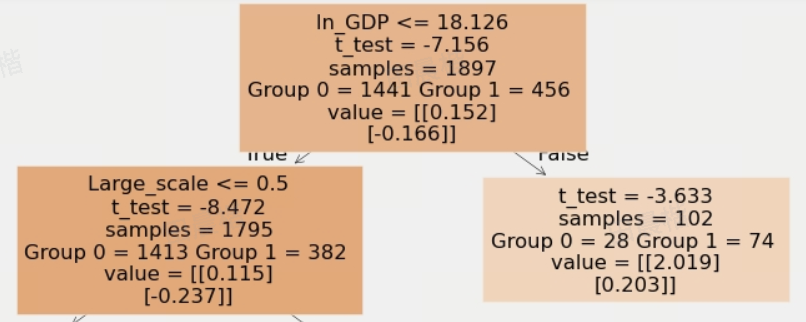
\includegraphics[width=0.8\textwidth]{beamerthemequito-light/Tree5.png}  
    \caption{An Unit of Causal Tree}
    \label{fig:Tree}  
\end{figure}
}

\frame{{Section 2}
{Regional Disparities \& Urban Characteristics}

We conduct the heterogeneity analysis based on regional disparities and urban characteristics.

\begin{itemize}
    \item Regional Disparities
    \begin{itemize}
        \item[$\ast$] Regions: Based on official data on China's regional economic division released by NBS.
        \item[$\ast$] City Size: Large ($>3$ million population) vs. Small ($<3$ million population).
        \item[$\ast$] Administrative Levels: High-level (provincial capitals) vs. Low-level(other cities).
    \end{itemize}
\end{itemize}



\begin{itemize}
    \item Urban Characteristics
    \begin{itemize}
        \item[$\ast$] Human Capital: High-level (above average ratio of students in college to registered population) vs. Low-level.
        \item[$\ast$] Pollution: High-pollution (above average emissions) vs. Low-pollution.
    \end{itemize}
\end{itemize}
}

\frame{{Section 2}
{Qini}

\begin{figure}[H]
    \centering
    \begin{subfigure}[b]{0.45\textwidth}
        \centering
        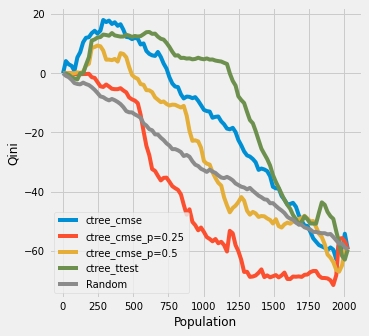
\includegraphics[width=\textwidth]{beamerthemequito-light/Qini1.png}
        \caption{Before PSM}
        \label{fig:Qini1}
    \end{subfigure}
    \hfill
    \begin{subfigure}[b]{0.45\textwidth}
        \centering
        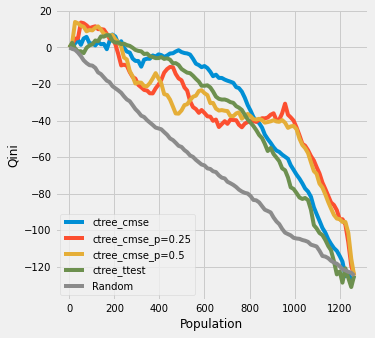
\includegraphics[width=\textwidth]{beamerthemequito-light/Qini2.jpg}
        \caption{After PSM}
        \label{fig:Qini2}
    \end{subfigure}
    \label{fig:Qini}
\end{figure}
}

\frame{{Section 2}
{Causal Forest}

\begin{figure}[H]
    \centering
    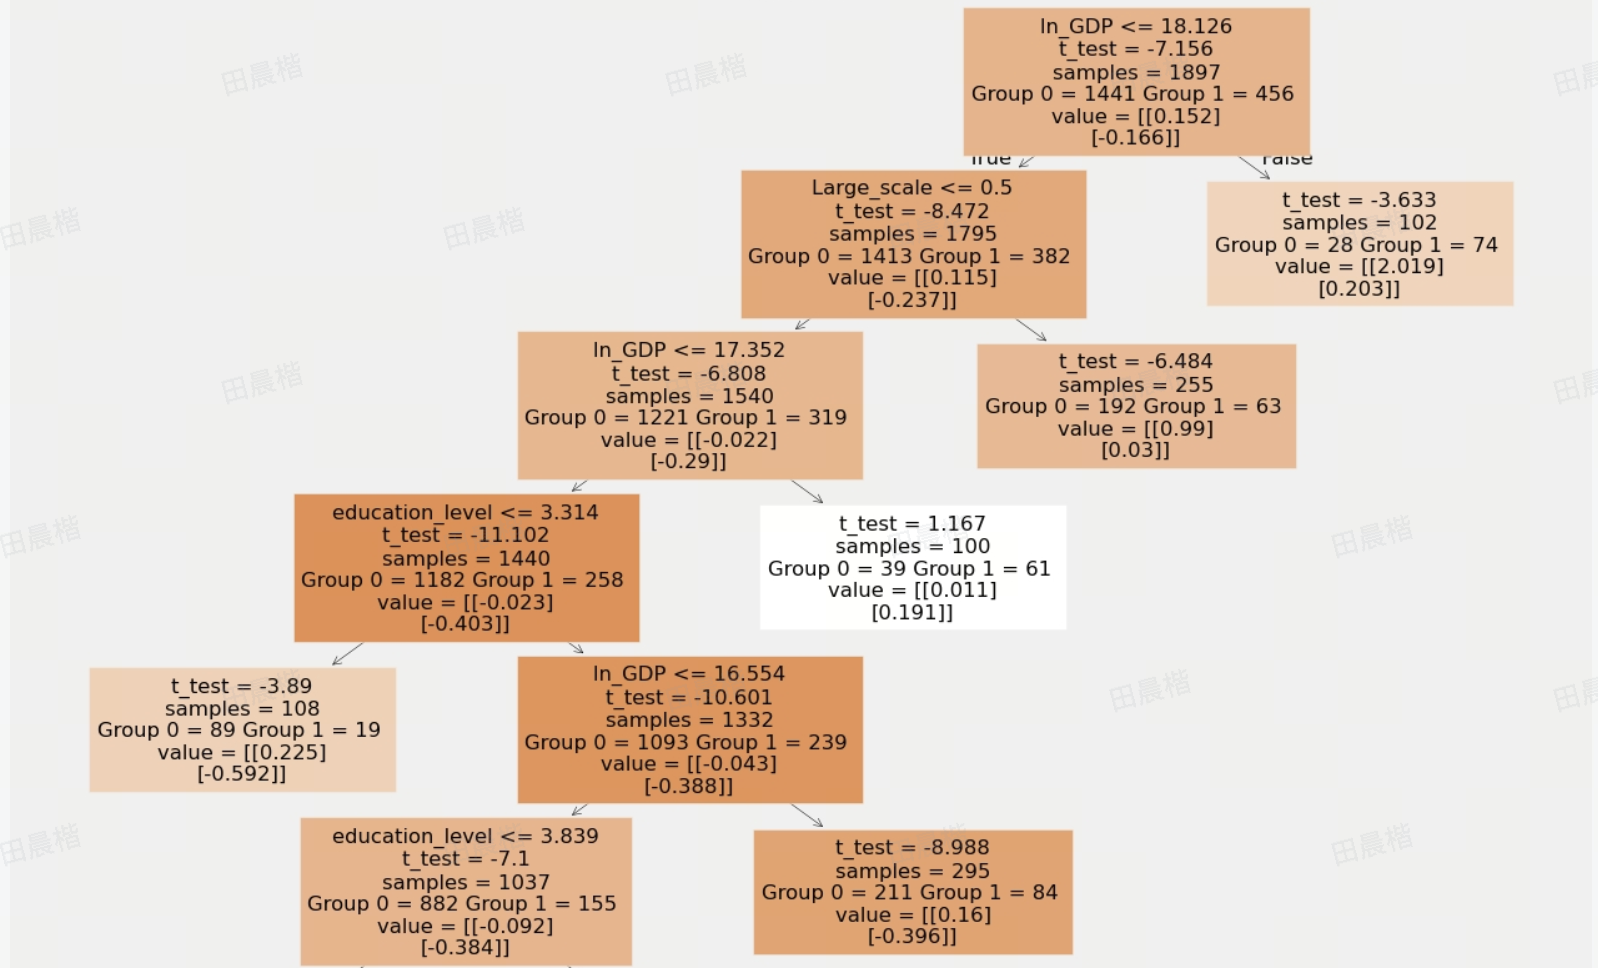
\includegraphics[width=0.6\textwidth]{beamerthemequito-light/Tree1.png}  
    \label{fig:Tree1}  
\end{figure}
}

\frame{{Section 2}
{Causal Forest}

\begin{figure}[H]
    \centering
    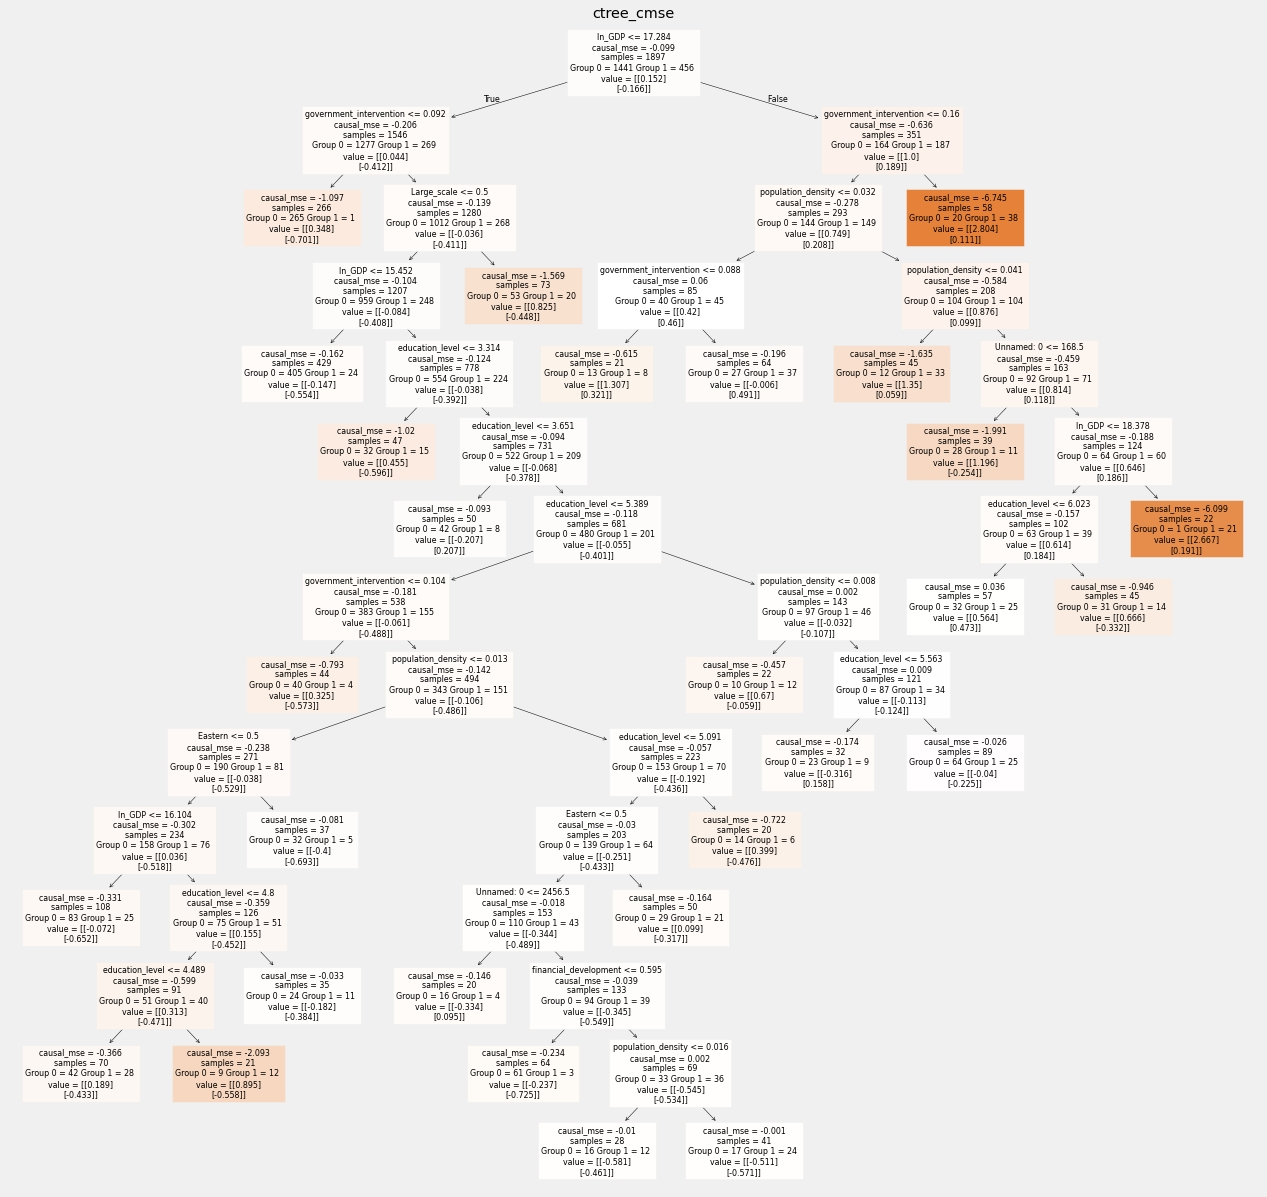
\includegraphics[width=0.6\textwidth]{beamerthemequito-light/Tree2.png}  
    \label{fig:Tree1}  
\end{figure}
}

\frame{{Section 2}
{Causal Forest}
\begin{figure}[H]
    \centering
    \begin{subfigure}[b]{0.45\textwidth}
        \centering
        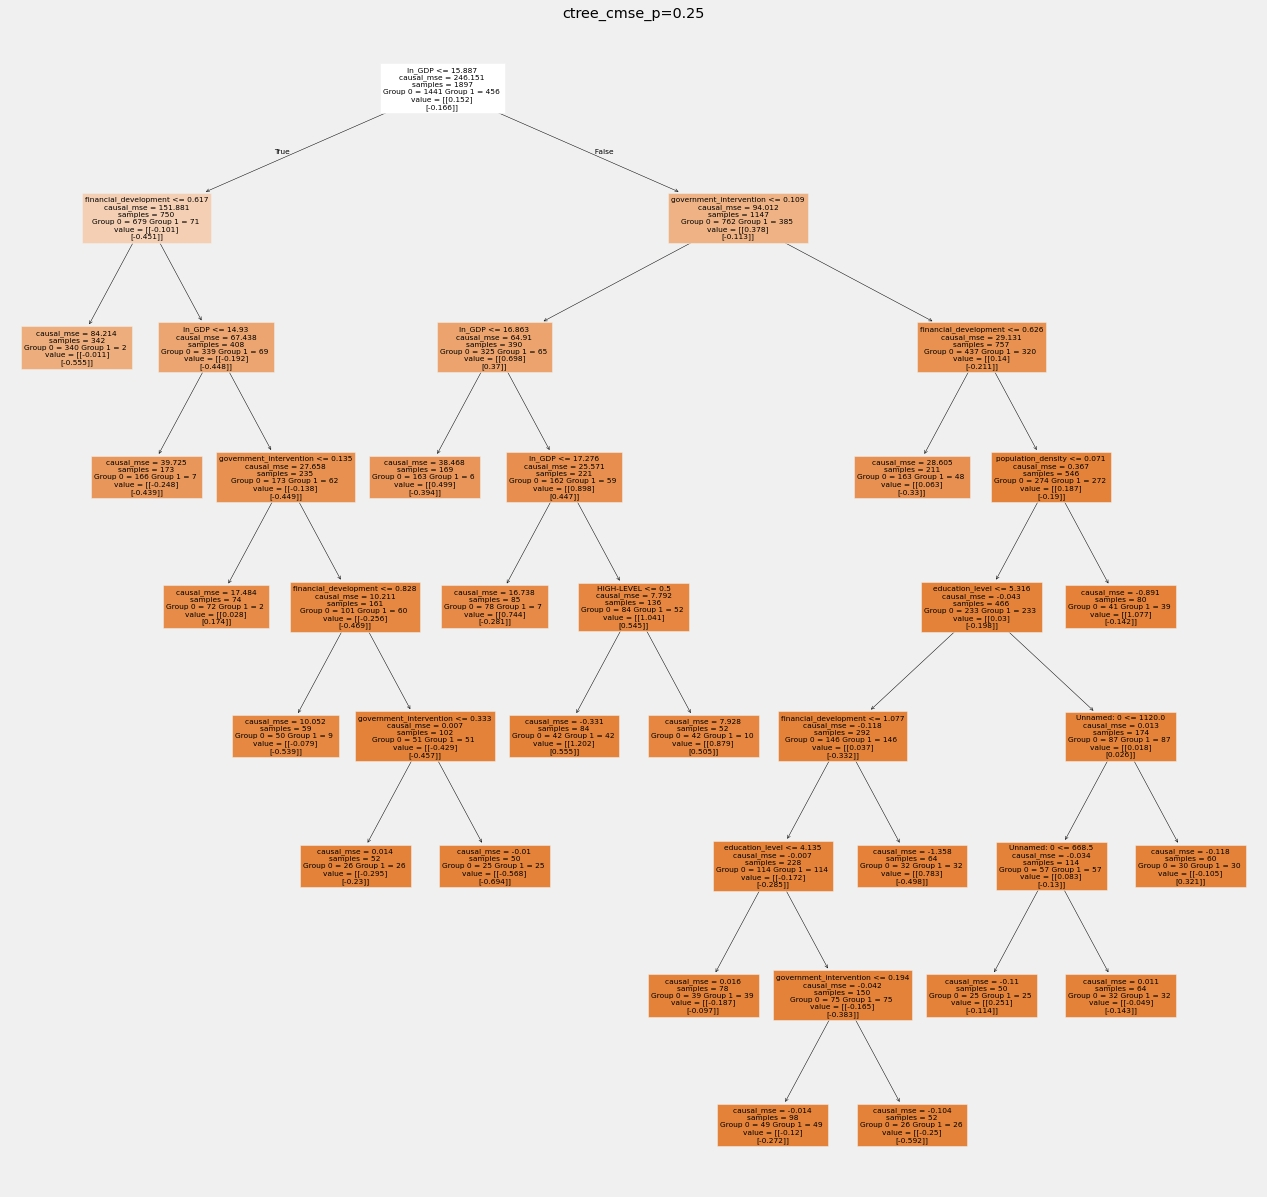
\includegraphics[width=\textwidth]{beamerthemequito-light/Tree3.png}
        \caption{$p=0.25$}
    \end{subfigure}
    \hfill
    \begin{subfigure}[b]{0.45\textwidth}
        \centering
        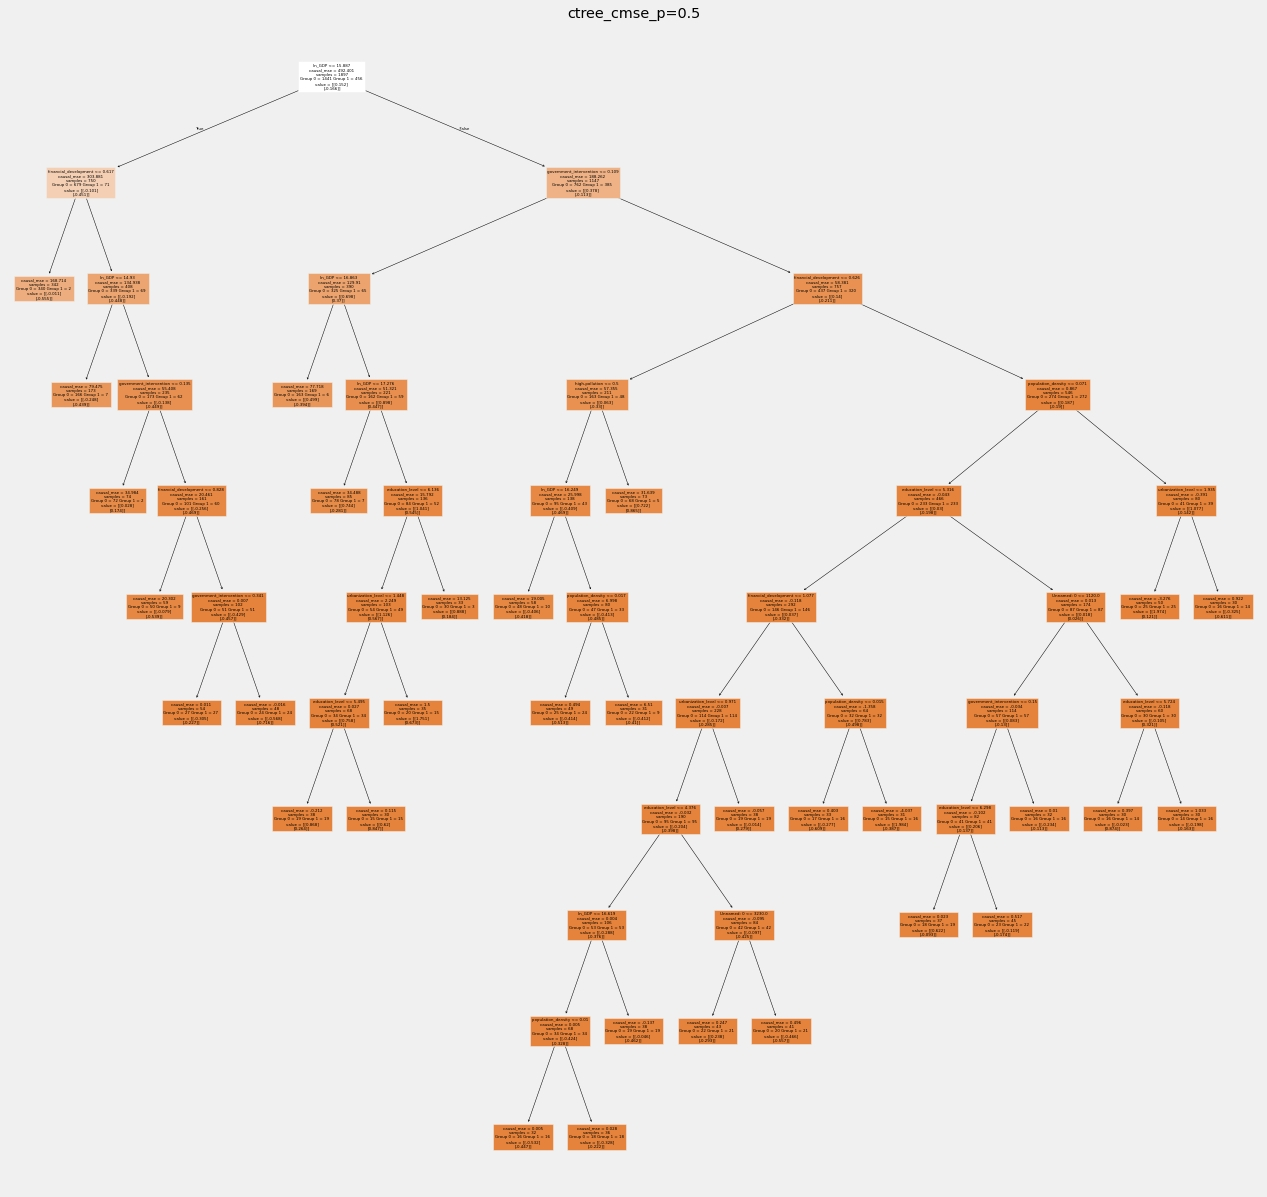
\includegraphics[width=\textwidth]{beamerthemequito-light/Tree4.png}
        \caption{$p=0.5$}
    \end{subfigure}
\end{figure}
}

\frame{{Section 2}
{Heterogeneity Analysis: Results}

\begin{figure}[H]
    \centering
    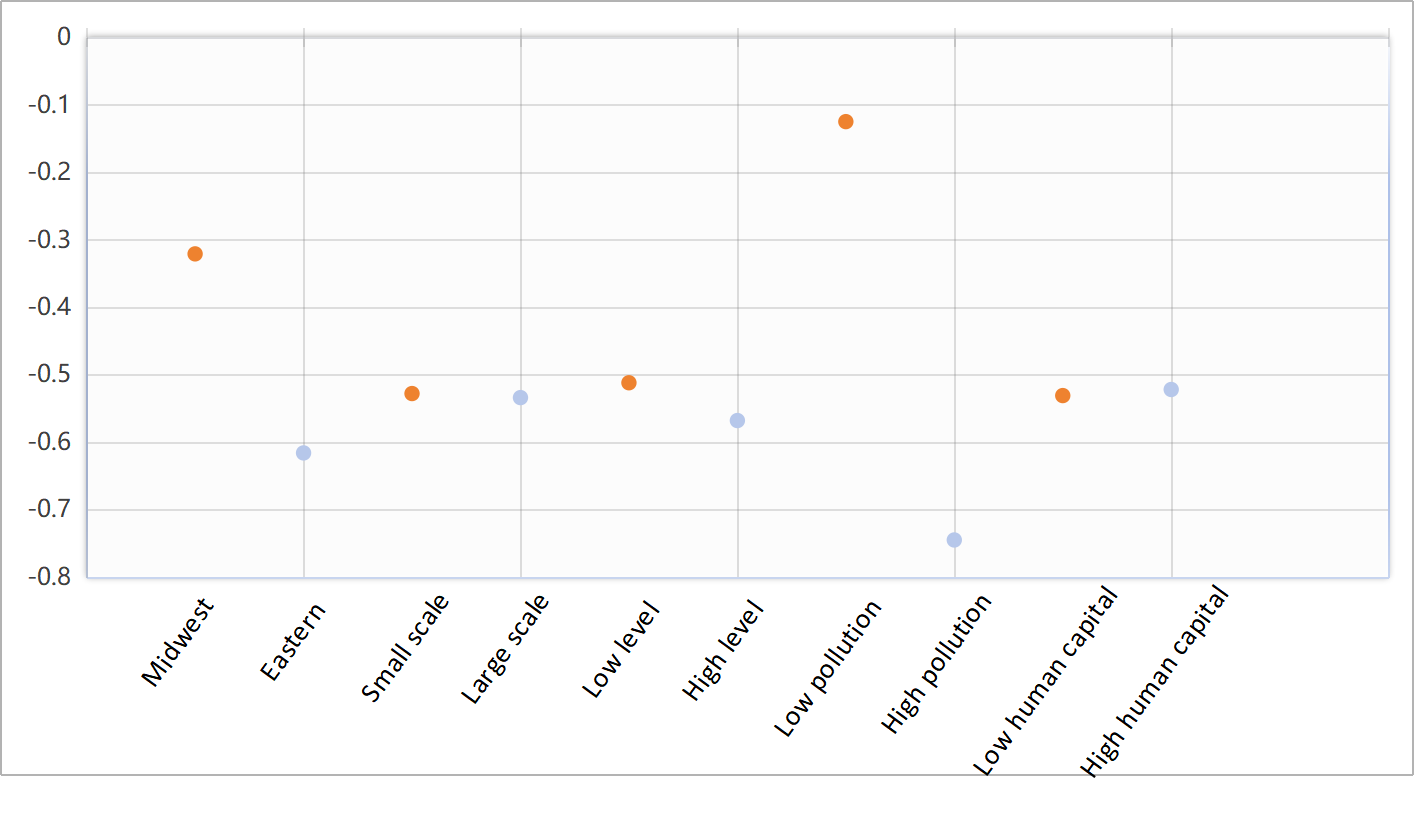
\includegraphics[width=0.8\textwidth]{beamerthemequito-light/Hetero.jpg}  
    \label{fig:hetero}  
\end{figure}
}

\frame{{Section 2}
{Heterogeneity Analysis: Results}

\begin{itemize}
    \item Most coefficients are around -0.5, aligned with the estimated results using DDML.
    \item Eastern cities outperform western cities, presumbly due to more efficient governments and better environmental awareness. 
    \item The estimated coefficient in highly polluted cities is much lower, suggesting the huge impact of SCC on environmental management where environmental issues are severe.
\end{itemize}
}
%_____________________________________________________
% 	References
\frame[allowframebreaks,noframenumbering]{{References}
{References}

\nocite{*}
\bibliographystyle{abbrvnat}
\bibliography{Biblio}
}

\frame{{CRediT}
{CRediT: Contribution Statement}

\begin{itemize}
    \item \textbf{Chenkai Tian 2211333}
    \item[$\ast$] \LaTeX(Slides \& Report), Methodology, Software, Validation, Visualization, Formal Analysis of Section 1(Entropy Weight Method, Baseline Regression, Parallel Trend Test, Placebo Test, Bacon Decomposition, PSM-DiD).
\end{itemize}

\begin{itemize}
    \item \textbf{Zeyu Li 2212026}
    \item[$\ast$] Methodology, Software, Validation, Visualization, Formal Analysis of PSM-DiD, Section2(Robustness Test, DDML, Causal Forest).
\end{itemize}

\begin{itemize}
    \item \textbf{Hanxi Cao 2213152}
    \item[$\ast$]Data Curation(Data Acquisition \& Preprocessing), Visualization, Report(Section 1).
\end{itemize}

\begin{itemize}
    \item \textbf{Le Xu 2212962}
    \item[$\ast$]Data Curation(Data Acquisition \& Preprocessing), Visualization, Report(Section 2).
\end{itemize}

}

\frame{

\centering
\Huge{Thank you!}

}
%____________________________________________________

\end{document}